\documentclass[11pt,reqno]{article}
\usepackage{amsmath,amssymb,mathrsfs,amsthm}
\usepackage[UTF8]{ctex}
%\usepackage{xeCJK}
%\setCJKmainfont{SimSum}

\usepackage{graphicx,cite,cases}
%\usepackage[pagewise]{lineno}\linenumbers
%\usepackage{refcheck}
\usepackage{xcolor}
\usepackage{bm}			% 公式加粗
\usepackage{tabularx}   % 绘制定宽表格
\usepackage{authblk}	% 添加更多作者信息
\usepackage{appendix} 	% 生成附录
\usepackage{listings}   % 附录里的代码, 支持语言高亮
\usepackage{hyperref}   % 超链接, 自动跳转
\usepackage{subfigure}  % 插入多张图片
\hypersetup{hypertex=true,	% 定义超链接效果
colorlinks=true,
linkcolor=blue,
anchorcolor=blue,
citecolor=blue}

\setlength{\topmargin}{-1.5cm}
\setlength{\oddsidemargin}{0.0cm}
\setlength{\evensidemargin}{0.0cm}
\setlength{\textwidth}{16.7cm}
\setlength{\textheight}{23cm}
\headheight 20pt
\headsep    26pt
\footskip 0.4in

%%%%% 关于公式编号问题 %%%%%
%统一用equation环境
%如果需要加括号用\begin{cases}
%如果公式过长需要分行用\begin{split}
%如果一个equation里面需要多个公式, emmm没研究过

\newtheorem{theorem}{Theorem}[section]
\newtheorem{corollary}[theorem]{Corollary}
\newtheorem{lemma}[theorem]{Lemma}
\newtheorem{proposition}[theorem]{Proposition}
\newtheorem{remark}[theorem]{Remark}
\newtheorem{definition}[theorem]{Definition}
\numberwithin{equation}{section}


\renewcommand{\d}{\,\mathrm d}
\usepackage{algorithm,algorithmicx}  %写伪代码
\usepackage{algpseudocode}			% 写伪代码
%%%%%% 算法部分改为中文显示 %%%%%%%%%
%%\floatname{algorithm}{算法}
\renewcommand{\algorithmicrequire}{\textbf{Input:}}
\renewcommand{\algorithmicensure}{\textbf{Output:}}

%% Ctrl+Alt+R 编译
%% Ctrl+Alt+V 打开文档

\begin{document}

\title{微分方程数值解计算实习Lecture 4}

\author{朱荃凡}
\affil{(吉林大学数学系计算唐班)}
\date{\today}

\maketitle

\vspace{50pt}

\section{问题重述}
用线性元在均匀网格下求解边值问题\eqref{Eqn11}的数值解:
\begin{equation}\label{Eqn11}
	\begin{split}
	&-y''+\dfrac{\pi^2}{4}y=\dfrac{\pi^2}{2}\sin\dfrac{\pi}{2}x,\ 0<x<1,\\
	&\ \ y(0)=0,\qquad y'(1)=0.
	\end{split}
\end{equation}
要求:
\begin{itemize}
	\item  画出数值解的图像
	\item 对$[0,1]$区间均匀剖分成$N=10,20,30,\cdots,200$份,计算数值解和真解
	 \[u*=\sin\dfrac{\pi}{2}x\]
	的$L^2$误差和$H^1$误差,计算其关于网格长度$h=1/N$的数值收敛阶.
	\item 计算系数矩阵的条件数, 并用loglog()函数作图表示.
\end{itemize}

\newpage

\section{算法设计}
考虑到可读性和泛化能力,该程序的主函数FEM\underline{\ }zqf由运行参数, 
计算有限元的函数run\underline{\ }main和一些列辅助
函数组成.运行参数包括带求函数所在区间,边值条件和网格剖分的数量和计算收敛阶时迭代次数.辅助函数
包括真解,基函数,右端函数$f(x)$,高斯积分公式等等.

重点来看run\underline{\ }main()函数,它包含如下几个部分:

\begin{itemize}
	\item 标准区间上高斯积分公式的选点和权重
	\item 生成刚度矩阵stiffnessMatrix()
	\item 生成右端项rightHands()
	\item 处理边值条件boundaryMatrix()
	\item 解方程组solveAF()
	\item 计算误差errorEstimate()
	\item 作图plotFigure()
\end{itemize}
接下来逐一解释每个部分的功能与作用.

\subsection{高斯积分公式的选点和权重}
由于使用有限元时已经对区间做过了一次剖分,在每个小区间数值积分就没有必要使用复化Simpson
公式,故而采取高斯积分公式是不错的选择.出于精度和计算量的考虑,这里选取了五点高斯积分公式,其对应的节点和权重分别是
\begin{equation}
	\begin{split}
		&positions=[-0.9061798,-0.5384693,0,0.5384693,0.9061798]\\
		&weights=[0.2369269;0.4786287;0.5688889;0.4786287;0.2369269]
	\end{split}
\end{equation}
想要得到任意小区间上的积分值,首先要做一个仿射变换,把$[-1,1]$区间上的节点变换到
对应区间上的节点.然后带入被积分函数中得到函数值.最后再通过一个高斯积分函数得到结果.

\subsection{生成刚度矩阵stiffnessMatrix()}
设网格剖分后节点$x_i$处的基函数是
\begin{equation}
	\varphi_i(x)=\left\{\begin{matrix}
		\dfrac{x-x_{i-1}}{h},&\ x_{i-1}\le x\le x_i,\\
		\dfrac{x_{i+1}-x}{h},&\ x_{i}\le x\le x_{i+1},\\
	   0,&others.
	   \end{matrix}\right.
\end{equation}
需要注意的是在区间端点处的基函数只有半支.

再设由方程\eqref{Eqn11}方程得到的双线性形式
\begin{equation}
	a(u,v)=\int_0^1(u'v'+\dfrac{\pi^2}{4}uv)\d x.
\end{equation}
那么刚度矩阵中的元素$a_{ij}$可表示成
\begin{equation}
	a_{ij}=\int_0^1(\varphi_i'\varphi_j'+\dfrac{\pi^2}{4}\varphi_i\varphi_j)\d x.
\end{equation}

但是直接生成全矩阵并不是一个很好的方式,我们可以逐区间来看.首先生成一个
$(N+1)\times(N+1)$的零矩阵$A$,然后考虑每个区间上的单元矩阵.
在区间$I_j=[x_{j-1,x_j}]$上,仅涉及到两个基函数$\varphi_{j-1},\varphi_j$和四个矩阵元素
$A_{j-1,j-1},A_{j-1,j},A_{j,j-1}$和$A_{jj}$.具体来说,对矩阵元素的操作可表示为
\begin{equation*}
	\begin{split}
		&\qquad\quad A_{j-1,j-1}=A_{j-1,j-1}+a,\qquad A_{j,j}=A_{j,j}+a,\\
		&\qquad\quad A_{j-1,j}=A_{j-1,j}+b,\qquad A_{j,j-1}=A_{j,j-1}+b,\\
		&a=\int_{x_{j-1}}^{x_j}\left[(\varphi_{j}')^2+
		\dfrac{\pi^2}{4}\varphi_{j}^2\right]\d x,\ 
		b=\int_{x_{j-1}}^{x_j}\left[\varphi_{j}'\varphi_{j-1}'+
		\dfrac{\pi^2}{4}\varphi_{j}\varphi_{j-1}\right]\d x,
	\end{split}
\end{equation*}
通过计算可以得到
\[a=\dfrac{1}{h}+\dfrac{\pi^2}{12},\quad b=-\dfrac{1}{h}+\dfrac{\pi^2}{24}\]
该数值与区间无关,因而可以简单地使用一个for循环实现,最终我们就得到了刚度矩阵A.

\subsection{生成右端项rightHands()}
生成右端项F时,采取和上述矩阵类似的方法.首先生成一个$N+1$列的零向量$F$,然后
在区间$I_j=[x_{j-1},x_j]$上,
\begin{equation}
	\begin{split}
		&F_{j-1}=F_{j-1}+\int_{x_{j-1}}^{x_j}f(x)\varphi_{j-1}(x)\d x,\\
		&F_{j}=F_{j}+\int_{x_{j-1}}^{x_j}f(x)\varphi_{j}(x)\d x.
	\end{split}
\end{equation}
此处直接采用数值积分公式即可.

\subsection{处理边值条件boundaryMatrix()}
在编程课上的时候,我和其他同学有过讨论:由于Dirichlet边值条件,
所以我们已经知道了$y_0$的取值, 所以到底是要解一个$N\times N$的系数矩阵,还是解一个
$(N+1)\times(N+1)$的系数矩阵.我个人的想法是解$(N+1)\times(N+1)$的,这样可以把生成
矩阵和处理边值条件独立开来,降低程序的耦合度.对于不同的边值问题也方便修改.

\subsubsection{Dirichlet边值条件}
处理Dirichlet边值条件$y(0)=0$总共有三种可选方法:
\begin{itemize}
	\item 直接把矩阵的第一行元素和对应右端项清零,然后令$A_{00}=1.$
	\item 删掉矩阵的第一行和第一列,和右端项的第一行.解完方程组以后再把$y_0=0$补回去.
	\item 直接令$A_{00}$和为一个超级大的数(例如说$10^{15}$),这样的话第一列
	其他矩阵元素对$y_0$的影响就很小,解方程即可.
\end{itemize}
我在程序中采取了第一种方法.

\subsubsection{Neumann边值条件}
处理Neumann边值条件只用修改右端项
\begin{equation}
	F_j=F_j+p(b)\beta\varphi_j(b),\quad j=0,1,\cdots,n.
\end{equation}
而事实上只修改了第$n+1$个方程的右端项,因为当$j=0,1,\cdots,n-1$时,\ $\varphi_{j}(b)=0.$

\subsection{解方程组solveAF()}

直接解方程组$y=A\backslash F$.

\subsection{计算误差errorEstimate()}
计算$L^2$误差时先在每个区间上对真解与数值解之差的绝对值用高斯积分公式,然后求和.
事实上我选用了$H^1$半模,也就是真解与数值解导数之差绝对值的$L^2$模来代替$H^1$模,
这并不会影响误差的收敛速度.

如果不想用for循环的话,也可以使用矩阵来储存节点坐标,其中矩阵的每一行表示小区间上
的高斯积分节点.最后再用sum()函数求和.这样做的好处是可以提升程序的运行速度.

\subsection{作图plotFigure()}
画出对应图像即可.

\newpage

\section{程序结果}
\subsection{数值解图像}
这里分别展示剖分数$N=10$和$N=50$时的图像,其中橙色实线表示真解,蓝色点表示数值解. 
即使是$N=10$时,线性有限元的计算结果   依旧相当好.:\\[-20pt]
\begin{figure}[h]
	\centering
	\subfigure{
	  \label{fig:subfig1}
	  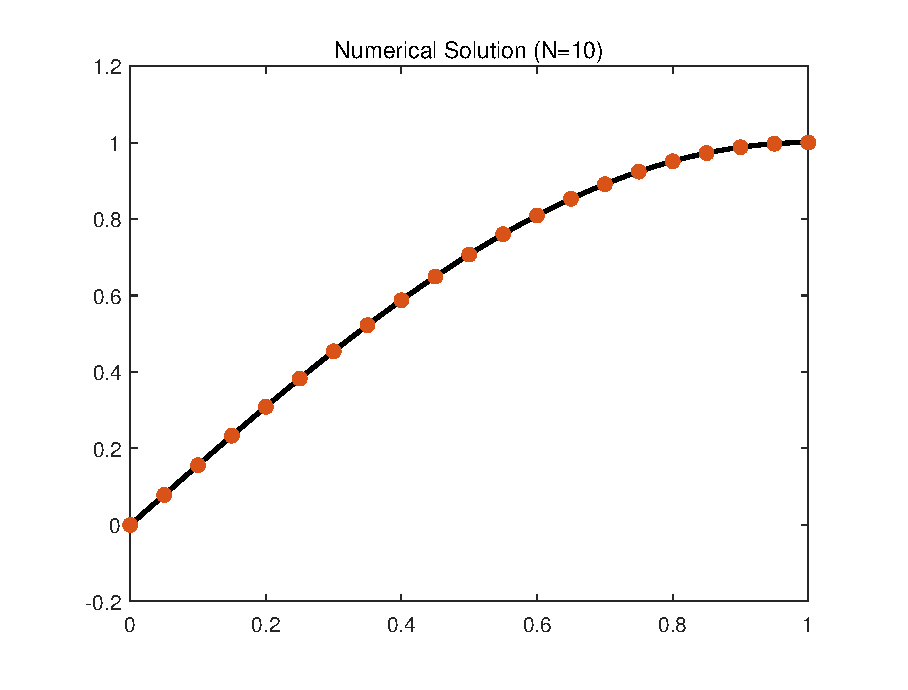
\includegraphics[width=0.48\textwidth]{N=10}}
	\subfigure{
	  \label{fig:subfig2}
	  \includegraphics[width=0.48\textwidth]{N=50}}
	  \caption{真解和数值解}
	\label{fig:subfigure}
\end{figure}

\subsection{误差和收敛阶}
接下来计算画出和收敛阶, 从图二图三中可以看出$H1$误差的收敛速度是$o(h)$,\ $L2$误差的收敛速度是$o(h^2)$,这与
理论是相符合的.
\begin{figure}[h]
	\centering
	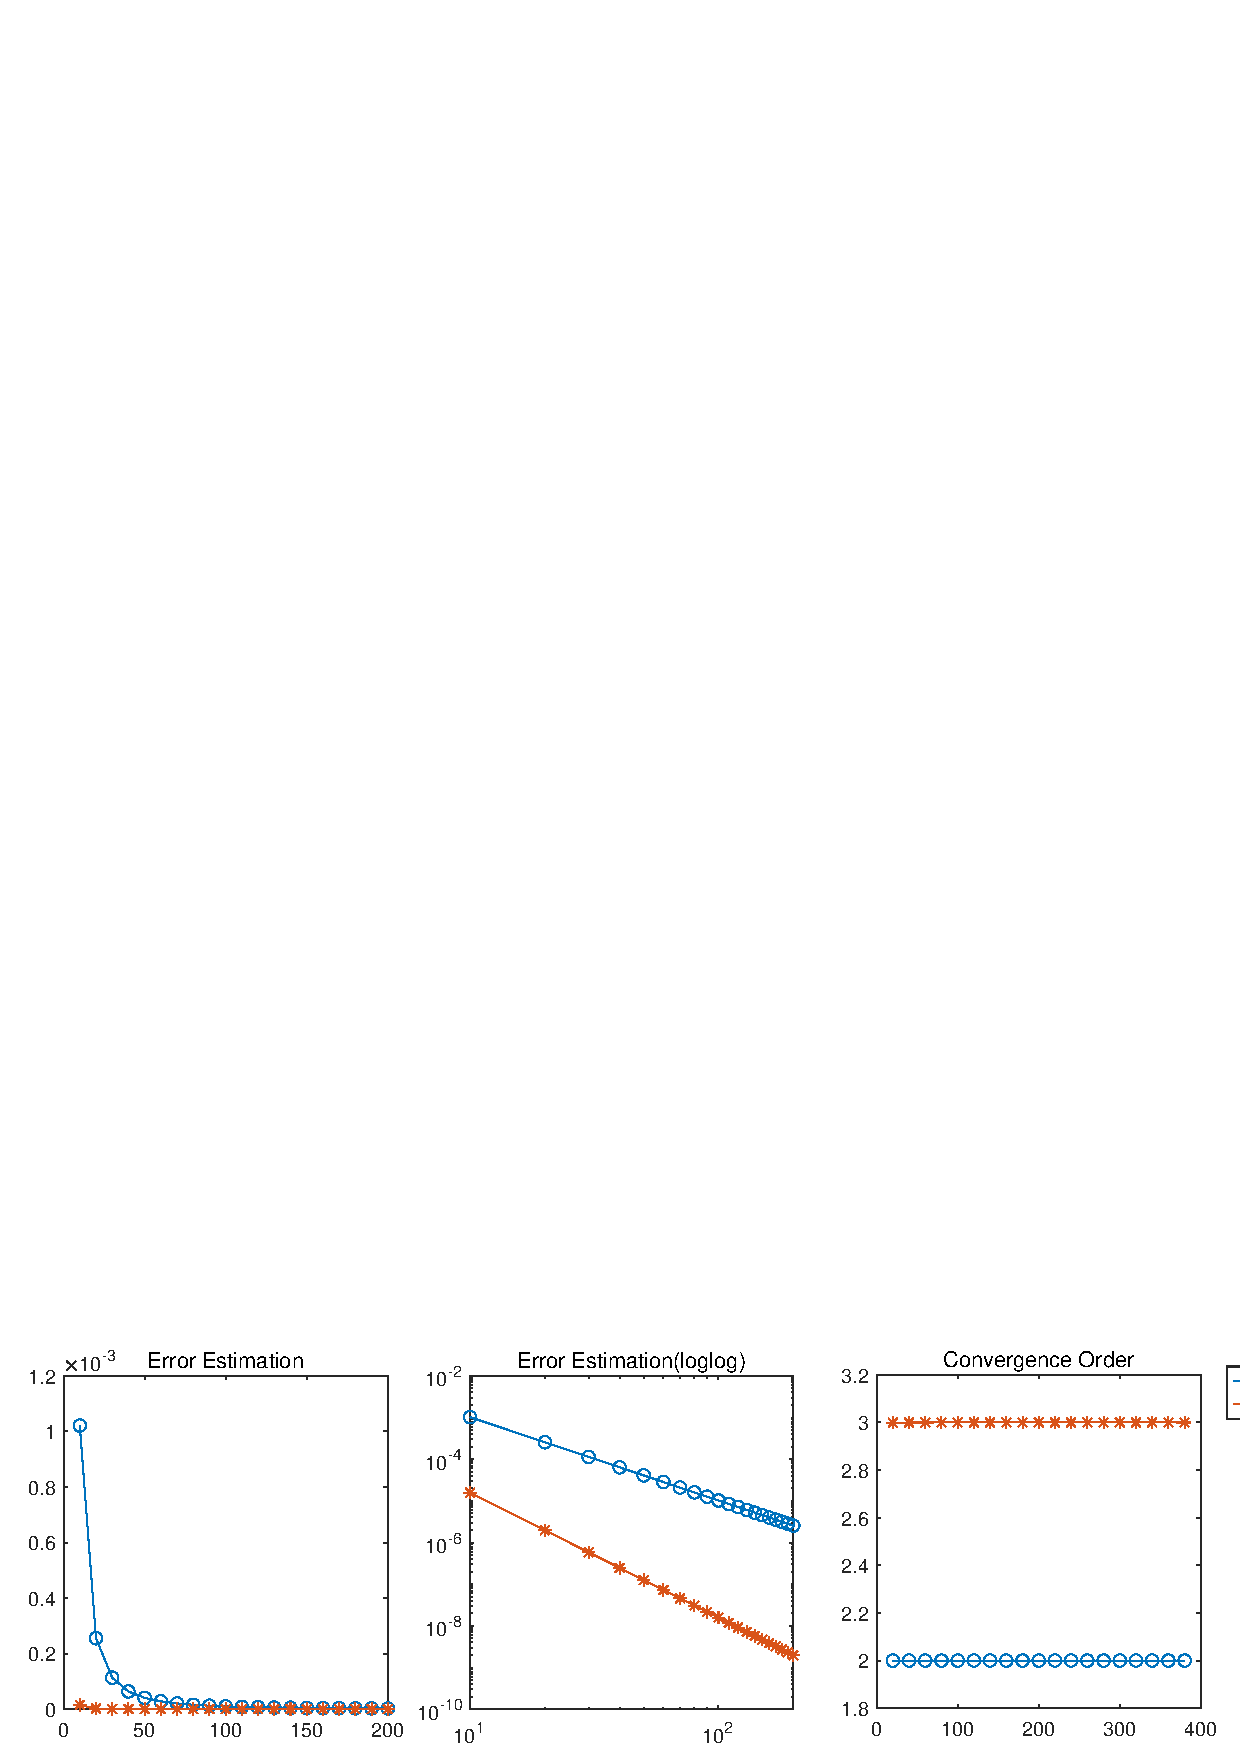
\includegraphics[width=\textwidth]{Error.jpg}
	\caption{误差和收敛阶}
\end{figure}

\newpage

\subsection{矩阵条件数}
最后是刚度矩阵的条件数$Cond(A)$. 假设$Cond(A)$的发散速度为
\begin{equation}
	Cond(A)=CN^\alpha,
\end{equation}
其中$N$为剖分数.对于不同的$N_1,N_2$有
\begin{equation}
	\alpha=\frac{\log{Cond(A_1)}-\log{Cond(A_2)}}{\log(N_1)-\log(N_2)}.
\end{equation}

于是我们画出如下的图像,其中图一是矩阵条件数与节点数量的双对数图,图二是发散阶.
\begin{figure}[h]
	\centering
	\includegraphics[width=\textwidth]{MatCon.jpg}
\end{figure}






\end{document}
